\chapter{Transverse Asymmetry}
The beam normal single spin asymmetry (BNSSA, also known as the transverse single spin asymmetry
or transverse asymmetry) is different from the PV asymmetry, it is purely 
EM and therefore parity-conserving. It arises from the interference
between the one-photon and two-photon exchanges (OPE and TPE), therefore it is sensitive 
to the TPE amplitude. By measuring it, we can probe the strength of the TPE, an 
important part of the electron elastic scattering that may explain the myth
of the proton radius: the radius difference between measurements with different methods.

The transverse asymmetry is also an important systematic uncertainty to the PV 
asymmetry measurement, because there is always some residual transverse polarizations
in the electron beam. With $\CA_n \sim \alpha_{EM}m_e/E_e$, its magnitude of $10^{-5}$ (10~ppm)
for a GeV level electron beam is much larger than $\CA_{\text{PV}}$, so a complete 
understanding and precise measurement of the transverse asymmetry is needed
to ensure the accuracy of $\CA_{\text{PV}}$.

Being a routine and bonus of a PV experiment, PREX-I also measured the transverse
asymmetry of some nuclei, namely ${}^{1}$H, \He, \C and \Pb. Surprisingly, PREX-I
saw a zero transverse asymmetry in \Pb, while the transverse asymmetries of other 
light nuclei agree with theoretical predictions, as shown in 
Fig.~\ref{fig:PREX-I_AT}. One of the reason for PREX-II is that we want to
verify the zero measurement in \Pb, which is still a puzzle to physicists.
\begin{figure}[!h]
    \centering
    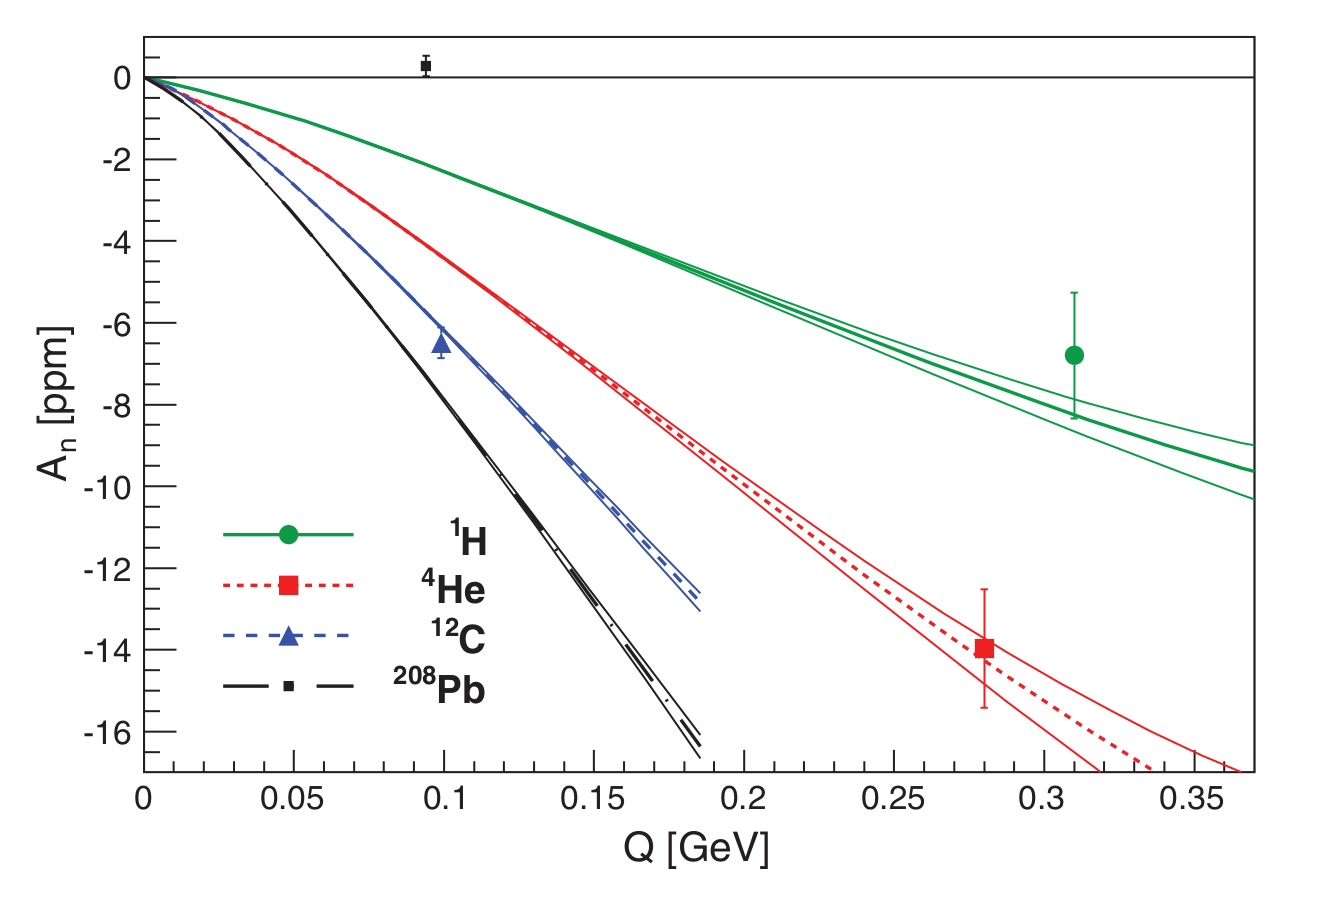
\includegraphics[width=0.5\linewidth]{PREX-I_AT}
    \caption{Transverse asymmetry measured in PREX-I \cite{PhysRevLett.109.192501}.}
    \label{fig:PREX-I_AT}
\end{figure}

As its name implies, BNSSA depends on only one spin, either the target or the
electron beam. A polarized electron beam is better than a polarized target in that 
it is hard to polarize nuclei, especially heavy nuclei.

%%%%%%%%%%%%%%%%%%%%%%%%%%%%%%%%%%%%%%%%%%%%%%%%%%%%%%%%%%%%%%%%%%%%%%%%
\section{Motivation for the Transverse Asymmetry}

%%%%%%%%%%%%%%%%%%%%%%%%
\subsubsection{The Scattering Theory}
Consider the scattering of a free ($t_0 \rightarrow -\infty$) particle from a 
time independent potential $V(\vec{r})$, 
which decays quickly as $r \rightarrow \infty$. The evolution from the free initial state
$\ket{i}$ is denoted as $\ket{\psi(t)}_S$ (under the Schr\"odinger picture and $\hbar = 1$):
\begin{equation}
    \ket{\psi(t)}_S = U(t)\ket{\psi(t_0)} = \lim_{t_0 \rightarrow -\infty}U(t, t_0)\ket{i}
\end{equation}
where $U(t, t_0)$ is the evolution operator:
\begin{equation}
    U(t, t_0) = \exp(\frac{1}{i}(H_0 + V)(t - t_0)) = \exp(-i(H_0 + V)(t-t_0))
\end{equation}
$H_0$ is the free Hamiltonian and $H = H_0 + V$ is the complete Hamiltonian
with the interaction term. 

The projection of $\psi(t)$ to a free final state $\ket{f}$ defines the so called
S-matrix (the order of the subscripts matters):
\begin{equation}
    S_{if} \equiv \lim_{t\rightarrow +\infty}\bra{f}\ket{\psi(t)} 
    = \lim_{t\rightarrow\infty} \lim_{t_0 \rightarrow -\infty} \bra{f} U(t, t_0) \ket{i}
\end{equation}
which defines the S operator:
\begin{equation}
    S_{if} = \bra{f} S \ket{i} \Longrightarrow S = U(+\infty, -\infty)
\end{equation}

The S-matrix describes the scattering amplitude from a free initial state $\ket{i}$
to a free final state $\ket{f}$. Conservation of the probability indicates
unitary of the S matrix:
\begin{equation}
    S^\dag S = \sum_f |\bra{f} U(+\infty, -\infty) \ket{i}|^2 = 1
\end{equation}

It is easier to evaluate $U(t)$ in the interaction picture. Define
\begin{equation}
    \ket{\psi(t)}_I \equiv \exp(-\frac{1}{i}H_0 t) \ket{\psi(t)}_S 
    = \exp(iH_0 t) \exp(-i (H_0 + V) t)\ket{i}
\end{equation}
The subscript I and S denote the interaction and Schr\"odinger picture respectively.
The evolution of $\ket{\psi(t)}_I$ is:
\begin{equation}
    \begin{aligned}
	\frac{d}{dt}\ket{\psi(t)}_I 
	&= \left[ \exp(i H_0 t) (iH_0) \exp(-i (H_0 + V) t)
	+ \exp(i H_0 t) (-i)(H_0 + V) \exp(-i (H_0 + V) t) \right] \ \ket{i}  \\
	&= -i\ \exp(i H_0 t)\ V \ \exp(-i (H_0 + V) t) \ket{i}   \\
	&= -i \exp(iH_0 t) V \exp(-iH_0 t) \cdot \exp(iH_0 t) \exp(-i(H_0 + V)t) \ket{i}   \\
	&= -i V_I(t) \ket{\psi(t)}_I
    \end{aligned}
    \label{eq:interaction_evolution}
\end{equation}
where $V_I(t) = \exp(iH_0t)V\exp(-iH_0t)$ is the time dependent interaction term.
Eq.~\ref{eq:interaction_evolution} leads to the Dyson series:
\begin{equation}
    U(t, t_0) = 1 - i\int_{t_0}^t dt_1 V_I(t_1) U(t_1, t_0) = \sum_{n=0}^\infty \frac{(-i)^n}{n!}\int_{t_0}^t dt_1 \cdots \int_{t_0}^t dt_n T[V_I(t_1)\cdots V_I(t_n)]
    \label{eq:U_expansion}
\end{equation}
T means the time-ordering:
\begin{equation}
    T(V_I(t_1) V_I(t_2)) \equiv 
    \begin{cases}
	V_I(t_1)V_I(t_2)    & t_1 \le t_2   \\
	V_I(t_2)V_I(t_1)    & t_2 \le t_1   \\
    \end{cases}
\end{equation}

With Eq.~\ref{eq:U_expansion}, we have an iterative expression:
\begin{equation}
    \begin{aligned}
	\bra{f} U(t, t_0) \ket{i} 
	&= \bra{f}\ket{i} - i \bra{f} \int_{t_0}^t dt_1 V_I(t_1) U(t_1, t_0) \ket{i}	\\
	&= \delta_{if} - i\sum_m \int_{t_0}^t dt_1 \bra{f}\exp(iH_0 t_1) V \exp(-iH_0 t_1)(t_1)\ket{m} \bra{m} U(t_1, t_0) \ket{i} \\
	&= \delta_{if} - i\sum_m \bra{f}V\ket{m} \int_{t_0}^t dt_1 \exp(i(E_f - E_m)t_1) \bra{m}U(t_1, t_0)\ket{i}  \\
    \end{aligned}
    \label{eq:finite_S-matrix}
\end{equation}

Truncate Eq.~\ref{eq:finite_S-matrix} into the first order ($\bra{m} U(t_1, t_0) \ket{i} = \delta_{im}$)
and define $T_{if} = \bra{f} V \ket{i}$, we write:
\begin{equation}
    \bra{f} U(t, t_0) \ket{i} = \delta_{if} - iT_{if} \int_{t_0}^t dt_1 \exp(i(E_f - E_i)t_1)
\end{equation}
and 
\begin{equation}
    \begin{aligned}
	S_{if} &= \lim_{t\rightarrow +\infty}\lim_{t_0 \rightarrow -\infty} \bra{f} U(t, t_0) \ket{i}    \\
	    &= \delta_{if} - iT_{if} \int_{-\infty}^{\infty} dt_1 \exp(i(E_f - E_i)t_1)	\\
	    &= \delta_{if} + i2\pi\delta(E_f - E_i)T_{if}   \\
    \end{aligned}
\end{equation}
In the matrix form:
\begin{equation}
    S = 1 + i2\pi T
\end{equation}
S being unitary implies
\begin{equation}
    S^\dag S = (1 - i2\pi T^\dag) (1 + i2\pi T) = 1 + i2\pi(T - T^\dag) + (2\pi)^2 T^\dag T = 1
\end{equation}
which reads
\begin{equation}
    T - T^\dag = i (2\pi)T^\dag T = i(2\pi) T T^\dag
\end{equation}
In terms of the matrix element:
\begin{equation}
    \begin{gathered}
    \delta(E_f - E_i)(T_{if} - T^\dag_{if}) = \sum_m i2\pi\delta(E_f - E_m)\delta(E_m - E_i)T_{fm}T^\dag_{mi}	\\
    T_{if} - T^\dag_{if} = \sum_m i2\pi\delta(E_m - E_i)T_{fm}T^\dag_{mi} = ia_{if} \\
    \end{gathered}
\end{equation}
where 
\begin{equation}
    a_{if} = \sum_m (2\pi) \delta(E_m - E_i)T_{fm}T^\dag_{mi}
\end{equation}
is the absorptive part of the transition amplitude $T_{if}$. $\ket{m}$ extends
to all on-shell intermediate states.

The two parts of S are easy to understand.
The constant piece denotes the evolution of one free particle into another free
particle without any interactions; obviously, it can evolve only into itself.
The T matrix describes the interaction (transition amplitude) between the free
initial particle $\ket{i}$ and the free final particle $\ket{f}$, which tells
the interaction cross section.

A free particle state can be completely described by its momentum $\vec{p}$
(ignoring the spin for now). For an incoming electron $\ket{\vec{p}_i}$, the probability
to transform into the final state of $\ket{\vec{p}_f}$ is:
\begin{equation}
    dP = (phase\ space) \times (transition\ probability) = \frac{d\vec{p}_f}{(2\pi)^3} \times |S_{\vec{p}_i\vec{p}_f}|^2
\end{equation}
For a non trivial case of $\ket{f} \ne \ket{i}$, we have:
\begin{equation}
    S_{if} = i2\pi \delta(E_f - E_i)T_{if}
\end{equation}
The differential cross section will be:
\begin{equation}
    d\sigma = \frac{dP}{\CL \Delta t}
\end{equation}
where $\CL$ is the luminosity, indicating number of particles hitting 
the target per unit area per unit time, in our case of incoming plane wave, 
$\CL = \rho v = v$, and $\Delta t$ is the interaction time.
\begin{equation}
    d\sigma = \frac{1}{v\Delta t} \frac{d\vec{p}_f}{(2\pi)^3} 2\pi\delta(E_f - E_i) \left. 2\pi\delta(E_f - E_i)\right|_{E_f = E_i} |T_{if}|^2
\end{equation}
Transform one $\delta$ expression back to the integrating form: 
\begin{equation}
    \left. 2\pi\delta(E_f - E_i) \right|_{E_f = E_i} 
    = \int_{-\infty}^{+\infty} dt \left.\exp(-i(E_f - E_i)t)\right|_{E_f = E_i}
    = \int_{-\infty}^{+\infty} dt 
\end{equation}
Physically, we don't go back or into infinity in time, because the real particle
is a finite wave packet rather than a plane wave. The integration above should 
be finite and close to the interaction time
\begin{equation}
    \int_{-\infty}^{+\infty} dt \rightarrow \Delta t
\end{equation}
Thus we have a defined cross section
\begin{equation}
    d\sigma = \frac{1}{v} \frac{d\vec{p}_f}{(2\pi)^3} 2\pi\delta(E_f - E_i) |T_{if}|^2
\end{equation}
The cross section is proportional to $|T_{if}|^2$, as already known to us.


%%%%%%%%%%%%%%%%%%%%%%%%
\subsubsection{T-Symmetry}
Time symmetry is an important discrete symmetry, which states that physical laws should
keep unchanged under the time reversal operation. Time reversal is the operation
that flips the time arrow, so that time runs backward after time reversal. Obviously, 
vectors that are first order derivatives of time will also reverse sign, such
as the momentum, angular momentum and magnetic field.

Express the time reversal operation with QM:
\begin{equation}
    \ket{\tilde{\psi}} = \hat{\mathcal{T}} \ket{\psi} 
\end{equation}
where $\hat{\mathcal{T}}: t \rightarrow -t$ is the time reversal operator. 

In terms of the scattering discussed above, a particle will flip its momentum 
and spin (angular momentum) under the time reversal, and pick up a phase.
\begin{equation}
    \ket{\tilde{\psi}} = \hat{\mathcal{T}} \ket{\psi_\uparrow(\vec{k})} = \eta\ket{\psi_\downarrow(-\vec{k})}
\end{equation}
$\eta$ is the phase difference and $|\eta|^2 = 1$ (two times of the time reversal operation
should transform a state back to itself.). The the T matrix in terms of the 
time reversed states is:
\begin{equation}
    T_{\tilde{i}\tilde{f}} = \bra{\tilde{f}} V \ket{\tilde{i}}
\end{equation}

It is well known that the EM interaction is invariant under time reversal.
\begin{equation}
    |T_{if}|^2 = |T_{\tilde{f}\tilde{i}}|^2 
\end{equation}

With these concepts, one can also define the T-odd quantities which
are proportional to the difference of the magnitude of a normal T element and 
its time reversed version:
\begin{equation}
    \begin{aligned}
	\text{T-odd} &\propto |T_{if}|^2 - |T_{\tilde{i}\tilde{f}}|^2	\\
	    &= |T_{if}|^2 - |T_{fi}|^2	\\
	    &= |T_{if}|^2 - |T^\dag_{if}|^2	\\
	    &= |T_{if}|^2 - |T_{if} - ia_{if}|^2	\\
	    &= -i(T_{if}a^*_{if} - T^*_{if}a_{if}) - |a_{if}|^2	\\
	    &= 2\text{Im}(T_{if}a^*_{if}) - |a_{if}|^2
    \end{aligned}
    \label{eq:T-odd}
\end{equation}

%%%%%%%%%%%%%%%%%%%%%%%%
\subsubsection{Transverse Asymmetry}
Denote the incoming and outgoing transversely polarized electron as 
$\ket{\vec{k}}$ and $\ket{\vec{k}'}$, the scattering is shown in Fig.~\ref{fig:transverse_scattering}.
\begin{figure}[h!]
    \centering
    \begin{subfigure}[c]{0.4\linewidth}
	\begin{tikzpicture}[scale=0.8]
	    \begin{feynman}[transform shape]
		\vertex (i1) {$e^-$};
		\vertex [right=1.0cm of i1, inner sep=0pt] (spin) {$\odot$};
		\vertex [right=2.3cm of spin] (ip);
		\vertex [right=2.8cm of ip] (i2) {A};
		\vertex [above right = 2cm and 2cm of ip] (o1) {$e^-$};
		\vertex [below left = 2cm and 2cm of ip] (o2) {A};

		\diagram* { {[edge=fermion]
		    (spin) --[edge label=$\vec{k}$] (ip) [dot] --[edge label = $\vec{k}'$] (o1),
		    (i2) --[edge label=$\vec{p}$](ip) [dot] -- [edge label = $\vec{p}'$]  (o2)},
		    (i1) -- (spin)
		};
	    \end{feynman}
	\end{tikzpicture}
    \end{subfigure}
    \hspace{0.2 cm}
    \textbf{-}
    \hspace{0.5 cm}
    \begin{subfigure}[c]{0.4\linewidth}
	\begin{tikzpicture}[scale=0.8]
	    \begin{feynman}[transform shape]
		\vertex (i1) {$e^-$};
		\vertex [right=1.0cm of i1, inner sep=0pt] (spin) {$\otimes$};
		\vertex [right=2.3cm of spin] (ip);
		\vertex [right=2.8cm of ip] (i2) {A};
		\vertex [above right = 2cm and 2cm of ip] (o1) {$e^-$};
		\vertex [below left = 2cm and 2cm of ip] (o2) {A};

		\diagram* { {[edge=fermion]
		    (spin) --[edge label=$\vec{k}$] (ip) [dot] --[edge label = $\vec{k}'$] (o1),
		    (i2) --[edge label=$\vec{p}$](ip) [dot] -- [edge label = $\vec{p}'$]  (o2)},
		    (i1) -- (spin)
		};
	    \end{feynman}
	\end{tikzpicture}
    \end{subfigure}
    \caption{Feynman diagrams of a transversely polarized electron scatters off
    an unpolarized nuclear target in the COM frame. The vector in or out of the plane
    indicates the electron's spin direction.} 
    \label{fig:transverse_scattering}
\end{figure}

The transverse asymmetry will be:
\begin{equation}
    \CA_n \equiv \frac{N_{\uparrow} - N_{\downarrow}}{N_{\uparrow} + N_{\downarrow}} 
    = \frac{|T_{\uparrow}(\vec{k}, \vec{k}')|^2 - |T_{\downarrow}(\vec{k}, \vec{k}')|^2}{|T_{\uparrow}(\vec{k}, \vec{k}')|^2 + |T_{\downarrow}(\vec{k}, \vec{k}')|^2}
\end{equation}
where $T(\vec{k}, \vec{k}') = \bra{\vec{k}'} V \ket{\vec{k}}$ is the scattering
amplitude and the arrow subscript indicates electron's spin direction.
$T_\downarrow(\vec{k}, \vec{k}')$ is related to $T_\downarrow(-\vec{k}, -\vec{k}')$
by a rotation around the normal direction of the scattering plane, as shown in
Fig.~\ref{fig:rotation_plot}
\begin{figure}[h!]
    \centering
    \begin{subfigure}[c]{0.4\linewidth}
	\begin{tikzpicture}[scale=0.8]
	    \begin{feynman}[transform shape]
		\vertex (i1) {$e^-$};
		\vertex [right=1.0cm of i1, inner sep=0pt] (spin) {$\odot$};
		\vertex [right=2.3cm of spin] (ip);
		\vertex [right=2.8cm of ip] (i2) {A};
		\vertex [above right = 2cm and 2cm of ip] (o1) {$e^-$};
		\vertex [below left = 2cm and 2cm of ip] (o2) {A};

		\diagram* { {[edge=fermion]
		    (spin) --[edge label=$\vec{k}$] (ip) [dot] --[edge label = $\vec{k}'$] (o1),
		    (i2) --[edge label=$\vec{p}$](ip) [dot] -- [edge label = $\vec{p}'$]  (o2)},
		    (i1) -- (spin)
		};
	    \end{feynman}
	\end{tikzpicture}
    \end{subfigure}
    \hspace{0.2 cm}
    $\Longrightarrow$
    \hspace{0.5 cm}
    \begin{subfigure}[c]{0.4\linewidth}
	\begin{tikzpicture}[scale=0.8]
	    \begin{feynman}[transform shape]
		\vertex (i1) {$e^-$};
		\vertex [left=1.0cm of i1, inner sep=0pt] (spin) {$\odot$};
		\vertex [left=2.3cm of spin] (ip);
		\vertex [left=2.8cm of ip] (i2) {A};
		\vertex [below left = 2cm and 2cm of ip] (o1) {$e^-$};
		\vertex [above right = 2cm and 2cm of ip] (o2) {A};

		\diagram* { {[edge=fermion]
		    (spin) --[edge label=$\vec{k}$] (ip) [dot] --[edge label = $\vec{k}'$] (o1),
		    (i2) --[edge label=$\vec{p}$] (ip) [dot] -- [edge label = $\vec{p}'$] (o2)},
		    (i1) -- (spin)
		};
	    \end{feynman}
	\end{tikzpicture}
    \end{subfigure}
    \caption{Rotation by $\pi$ around the normal direction of the scattering plane.} 
    \label{fig:rotation_plot}
\end{figure}
\begin{equation}
    T_\downarrow(\vec{k}, \vec{k}') = e^{i\pi} T_\downarrow(-\vec{k}, -\vec{k}')
\end{equation}

Let $T_{if} = T_{\uparrow}(\vec{k}, \vec{k}')$, then $T_{\tilde{i}\tilde{f}} = T_\downarrow (-\vec{k}, -\vec{k}')$
and
\begin{equation}
    \begin{aligned}
	\CA_n &\approx \frac{|T_{\uparrow}(\vec{k}, \vec{k}')|^2 - |T_{\downarrow}(-\vec{k}, -\vec{k}')|^2}{2|T_{\uparrow}(\vec{k}, \vec{k}')|^2} \\
	    &= \frac{|T_{if}|^2 - |T_{\tilde{i}\tilde{f}}|^2}{2|T_{if}|^2}  \\
	    &= \frac{2\text{Im}(T_{if}a^*_{if}) - |a_{if}|^2}{2|T_{if}|^2}
    \end{aligned}
    \label{eq:transverse_asymmetry}
\end{equation}

We see that the transverse asymmetry is a T-odd quantity. For the EM interaction
\begin{equation}
    T_{if} \propto \alpha \qquad a_{if} \propto \alpha^2
\end{equation}
Because $\alpha \simeq \frac{1}{137}$ is small, we can expand Eq.~\ref{eq:transverse_asymmetry} 
in order of $\alpha$. To the lowest order
\begin{equation}
    \CA_n = 0
    \label{eq:AT_0}
\end{equation}
and to the first order 
\begin{equation}
    \CA_n = \frac{\text{Im}(T_{if}a^*_{if})}{|T_{if}|^2}
    \label{eq:AT_1}
\end{equation}

$T_{ij}$ represents the OPE interaction while $a_{ij}$ represents
the TPE interaction. So the physical interpretation of
Eq.~\ref{eq:AT_0} and \ref{eq:AT_1} is that the time symmetry requires 
the transverse asymmetry to be zero under the Born approximation (OPE only)
and the (lowest order) non-zero transverse asymmetry comes from the interference 
between OPE and TPE.
\begin{figure}[!h]
    \centering
    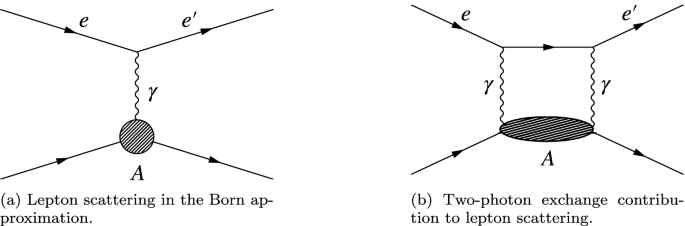
\includegraphics[width=0.8\linewidth]{at/OPE_n_TPE}
    \caption{Feynman diagrams of the OPE (left) and TPE (right).}
\end{figure}

%%%%%%%%%%%%%%%%%%%%%%%%%%%%%%%%%%%%%%%%%%%%%%%%%%%%%%%%%%%%%%%%%%%%%%%%
\section{Measurement of the Transverse Asymmetry: the Method}
The experimentally measured transverse asymmetry will be
\begin{equation}
    \CA_{\text{mea}} = \CA_n \vec{\CP}_e \cdot \hat{n} = \CA_n \CP_n \sin(\phi_s - \phi_e) = \CA_n \CP_n \sin\phi
    \label{eq:measured_AT}
\end{equation}
where $\vec{\CP}_e$ is the electron spin vector, whose magnitude is the polarization,
and $\CP_n$ being its transverse component,
$\phi_s$ being its angle w.r.t. the lab horizontal plane; 
$\hat{n} = \frac{\vec{k} \times \vec{k}'}{|\vec{k} \times \vec{k}'|}$ 
is the unit normal vector of the scattering plane and $\phi_e$ the angle between
the scattering plane and the horizontal plane. As shown in Fig.~\ref{fig:AT_scattering}.
So $\phi = \phi_s - \phi_e$ is the angle between the spin vector and the scattering plane.
\begin{figure}[h!]
    \centering
    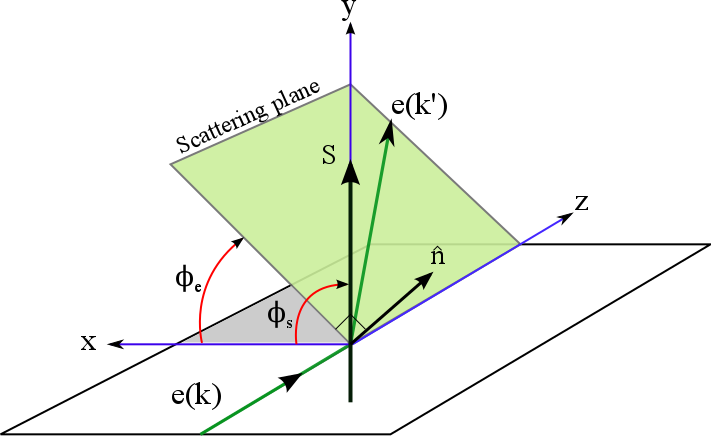
\includegraphics[width=0.7\linewidth]{AT_scattering}
    \caption{Schematic plot of the scattering of a transversely polarized electron.}
    \label{fig:AT_scattering}
\end{figure}

Eq.~\ref{eq:measured_AT} shows the angle dependence of the transverse asymmetry. 
Experimentally, it is convenient to select the angle $\phi$ being $90^\circ$. 
With the lab horizontal plane as the scattering plane, the electron spin will
be vertical, being perpendicular to the scattering plane, as done in PREX-II and CREX. 
Detailed dynamics for the AT measurement are listed in Table~\ref{tab:AT_dynamics}.

\begin{table}
    \centering
    \begin{tabular}{c c | c c c}
	\hline
	Exp (Energy)	& Target    & $\langle \theta \rangle ({}^\circ)$   & $\langle Q^2 \rangle \ (\mathrm{GeV}^2)$	& $\langle \sin\phi \rangle$	\\
	\hline
	\multirow{3}{*}{PREX-II (0.95~GeV)}
	    & \C    & 4.87  & 0.0067    & 0.967 \\ 
	    & \ca   & 4.81  & 0.0067    & 0.964 \\ 
	    & \Pb   & 4.69  & 0.0064    & 0.966 \\ 
	\hline
	\multirow{4}{*}{CREX (2.18~GeV)}
	    & \C    & 4.77  & 0.033	& 0.969 \\ 
	    & \ca   & 4.55  & 0.031	& 0.970 \\ 
	    & \Ca   & 4.53  & 0.031     & 0.970 \\ 
	    & \Pb   & 4.60  & 0.032     & 0.969 \\ 
	\hline
    \end{tabular}
    \caption{Dynamics of the AT measurement in PREX-II/CREX.}
    \label{tab:AT_dynamics}
\end{table}

To achieve the transverse polarization, a different configuration of the double 
wien filters is needed. Specifically, we just rotate the spin to the vertical 
direction using the vertical wien filter, the 
following rotations we do for the longitudinal polarization, as shown in 
Fig.~\ref{fig:double_wien_filter}, are omitted (the spin solenoid's rotating
angle is set to $~0^\circ$). Because the spin is parallel/anti-parallel
to the magnetic field in the accelerator arc area, there is no spin precession as in
the case of the longitudinal polarization. 

In terms of the measurement of the transverse polarization, neither Moller, nor Compton
polarimeter is used, because their analyzing powers go to 0 at the limit of transverse
polarization. Without a direct measurement of the polarization in the hall, 
we turn to the Mott polarimeter in the injector. 
As said above, the beam transportation from injector to Hall A
is symmetric and flat, which means the vertical component of the polarization
is preserved (can be safely assumed $>99.9\%$), so the measurement in the
injector can be used as that in the hall.

Except the difference in the configuration of the double wien filters, everything 
else is the same as in the case of the longitudinal polarization (the Compton Chicane
is off). 

%%%%%%%%%%%%%%%%%%%%%%%%
\subsubsection{Polarization Measurement}
The 5~MeV Mott polarimter is used to verify the transverse polarization,
which gives about 87\% transverse polarization for both PREX-II and CREX runs.
The Mott data is summarized in Table~\ref{tab:AT_Mott}.
% https://logbooks.jlab.org/entry/3781205, https://logbooks.jlab.org/entry/3718518, 
\begin{table}[!h]
    \begin{tabular}{c c c | c c | c}
	\hline
	exp & run & IHWP  & UD (\%)	& LR (\%)   & Vertical Pol (\%)	\\
	\hline
	\multirow{2}{*}{PREX-II}
	    & 8966  & OUT   & $0.0704732 \pm 0.435101$	& $-34.193 \pm 0.418556$	& -87.2048  \\
	    & 8967  & IN    & $0.421465 \pm 0.432328$	& $33.9616 \pm 0.419132$	&  86.6146  \\
	\hline
	\multirow{5}{*}{CREX}    
	    & 9081  & IN    & $-1.16128 \pm 0.334165$   & $-34.1276 \pm 0.325363$	& -87.0380  \\
	    & 9082  & OUT   & $-0.105704 \pm 0.328932$	& $34.0755 \pm 0.324116	$&  86.9051  \\
	    & 9083  & IN    & $-0.613295 \pm 0.333657$	& $-34.3502 \pm 0.32453	$& -87.6057  \\
	    & 9084  & OUT   & $-0.0248337 \pm 0.326988$	& $34.4674 \pm 0.318313	$&  87.9046  \\
	    & 9085  & IN    & $-1.15795 \pm 0.33341 $   & $-34.0401 \pm 0.32742	$& -86.8148  \\
	\hline
    \end{tabular}
    \caption{Mott measurements during PREX-II and CREX AT runnings. The Up-Down
    asymmetry measures the horizontal transverse polarization while the Left-Right
    asymmetry measures the vertical transverse polarization; The Mott analyzing 
    power is $\CA_{\text{Mott}} = 0.3921 \pm 0.0016$, so the vertical polarization is 
    $\frac{\CA_{\text{LR}}}{\CA_{\text{Mott}}}$.} 
    \label{tab:AT_Mott}
\end{table}

The actual value we use for the transverse asymmetry calculation is the 
average longitudinal polarization measured shortly before and after the AT runs, 
with confidence in our pretty wien filter settings and that the accelerator 
won't change the beam transverse polarization. 
The polarization result is shown in Table~\ref{tab:AT_polarization}
\begin{table}[!h]
    \centering
    \begin{tabular}{c | c c c}
    \hline
    Exp	& Compton (\%)	& Moller (\%)	& $P_n$ (\%) \\
    \hline
    PREX-II & $88.5533 \pm 0.447$   & $89.67 \pm 0.8$	& $89.7 \pm 0.8$  \\
    CREX    & $86.67 \pm 0.63$	& $86.897 \pm 0.778$	& $86.8 \pm 0.6$  \\
    \hline
    \end{tabular}
    \caption{Average Compton and Moller polarization measured near the AT runs. 
    The PREX-II AT uses only the Moller result while the CREX one uses the average value of the 
    Compton and the Moller measurements.}
    \label{tab:AT_polarization}
% FIXME why only the moller result for PREX-II
\end{table}

%%%%%%%%%%%%%%%%%%%%%%%%%%%%%%%%%%%%%%%%%%%%%%%%%%%%%%%%%%%%%%%%%%%%%%%%
\section{Data}

% how much data is needed?
We spent 1 (2) days in PREX-II (CREX) for the transverse asymmetry measurement,
and collected 25 (56) good AT runs in PREX-II (CREX).
% PREX-II: 20190813 - 20190814
% CREX: 20200210 - 20200212

\begin{table}[!h]
    \centering
    \begin{tabular}{c | c | c | c | l}
	\hline
	exp & target	& IHWP	& \# runs    & run number    \\
	\hline
	\multirow{6}{*}{PREX-II}    & \multirow{2}{*}{\C}   & IN    & 3	& 4106-4107, 4133    \\
	    &   & OUT   & 4 & 4108-4109, 4131-4132   \\
	    \cline{2-5}
	    & \multirow{2}{*}{\Pb}  & IN    & 7	& 4115-4119, 4129-4130  \\
	    &	& OUT	& 6 & 4110-4114, 4128   \\
	    \cline{2-5}
	    & \multirow{2}{*}{\ca}  & IN    & 3	& 4123-4125	\\
	    &	& OUT	& 2 & 4126-4127 \\
	\hline
	\multirow{8}{*}{CREX}	& \multirow{2}{*}{\Ca}	& IN	& 9 & 6344-6345,6354-6355,6380-6382,6407-6408\\
	    &	& OUT	& 10	& 6346-6348,6356-6357,6383-6385,6405-6406   \\
	    \cline{2-5}
	    & \multirow{2}{*}{\ca}	& IN	& 7 & 6351-6352,6394-6396,6401-6402	\\
	    &	& OUT	& 7 & 6349-6350,6398-6400,6403-6404	\\
	    \cline{2-5}
	    & \multirow{2}{*}{\C}	& IN	& 6 & 6361-6363,6389-6391	\\
	    &	& OUT	& 5 & 6359-6360,6386-6388	\\
	    \cline{2-5}
	    & \multirow{2}{*}{\Pb}	& IN	& 7 & 6367-6371,6377-6378	\\
	    &	& OUT	& 5 & 6372-6376 \\
	\hline
    \end{tabular}
    \caption{AT runs in PREX-II/CREX}
\end{table}

%%%%%%%%%%%%%%%%%%%%%%%%%%%%%%%%%%%%%%%%%%%%%%%%
\subsection{Data Analysis}
Using the data set after 2 respins and following the standard analysis procedure, 
the transverse asymmetry is extracted. As shown in Eq.~\ref{eq:measured_AT},
$\hat{n}$ of the scattering plane for LHRS and RHRS are opposite to each other,
so the measured transverse asymmetries have opposite sign in LHRS/RHRS. To
combine measurement from both arms, we use the asymmetry (double) difference, 
instead of the asymmetry average as in the main analysis. The asymmetry difference
is defined as (up to a `-' sign):
\begin{equation}
    \CA_{\text{dd}} = \frac{\CA_L - \CA_R}{2}
\end{equation}

% no beammod data
A simple cut of \verb|ErrorFlag == 0| is applied to select good quadruplets 
(in PREX-II, run 4112 is a long run with its data split into two rootfiles, the
second one contains only a small size of samples, therefore is ignored in our AT analysis.
Besides, the first minirun of run 4117 is removed due to the large charge asymmetry
in that minirun). The good quadruplets are first grouped into miniruns, 
the average of these miniruns for each target will be what we wanted. 
One can also extract the transverse asymmetry from the histogram filled with
all quadruplets -- the mulplot, whose mean value will be our final result. 
Statistically, there is no difference between these two methods,
they use the same data set and weight each sample equivalently, so they can
be used to cross check each other. The mulplots and minirun average plots for
CREX \Ca are shown below in Fig.~\ref{fig:AT_crex_Ca48_mulplot} and 
Fig.~\ref{fig:AT_crex_Ca48_miniruns}, as an example.

\begin{figure}[!h]
    \centering
    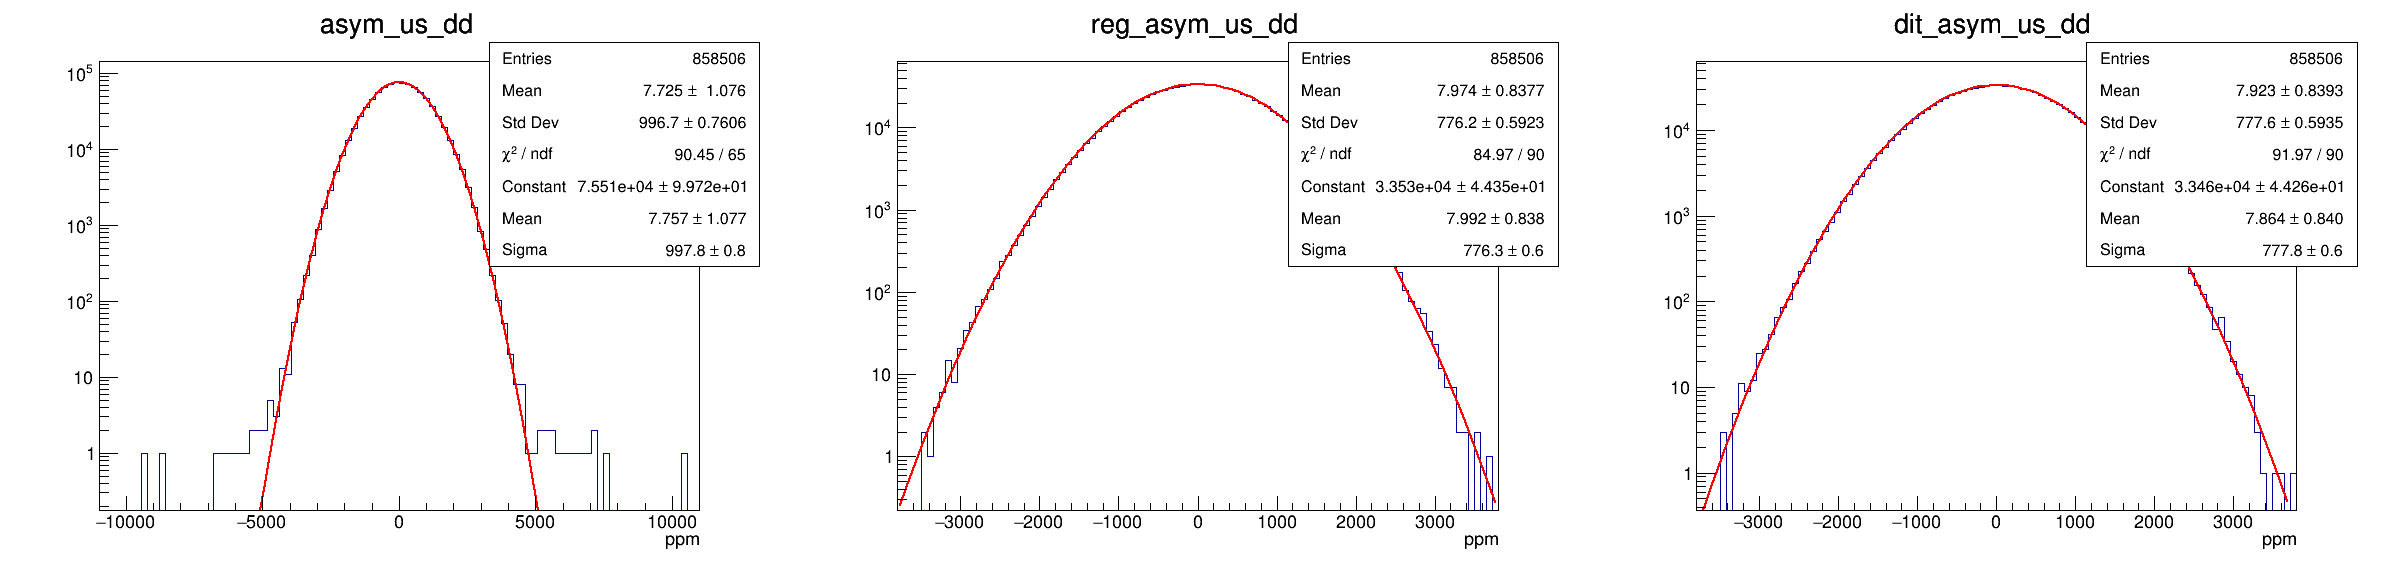
\includegraphics[width=\linewidth]{at/mulplot_Ca48}
    \caption{Mulplots for CREX \Ca. The red line is a Gaussian fit. One can clearly 
    see how the false asymmetry correction reduces the width of the distribution (note that
    the first plot has a larger X-range than the other two).}
    \label{fig:AT_crex_Ca48_mulplot}
\end{figure}

\begin{figure}[H]
    \centering
    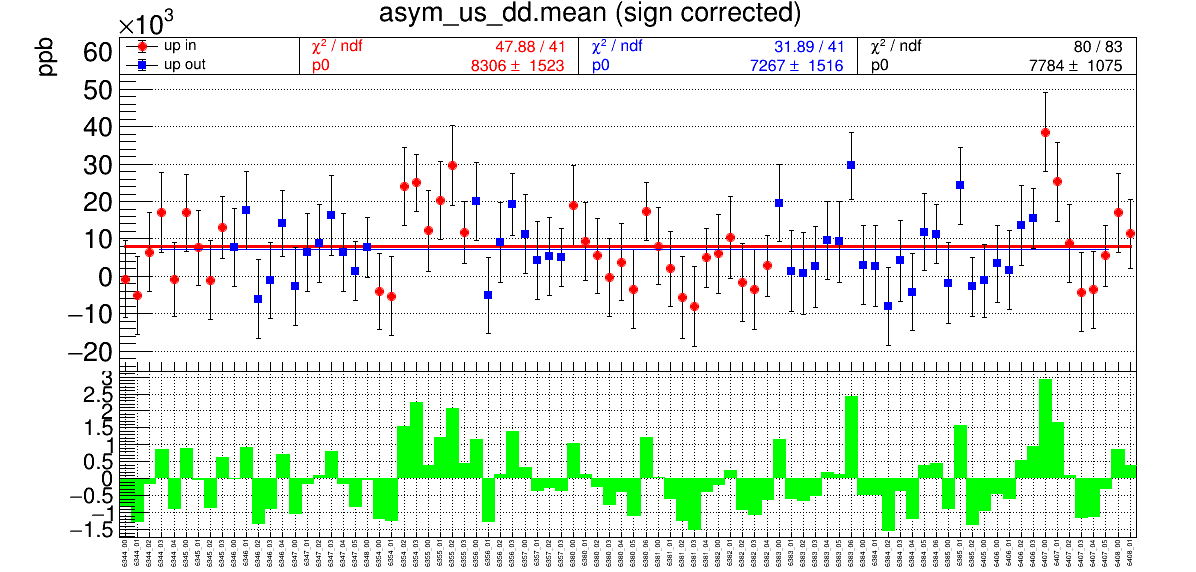
\includegraphics[width=0.9\linewidth]{at/mini_Ca48_asym_us_dd.mean.png}
    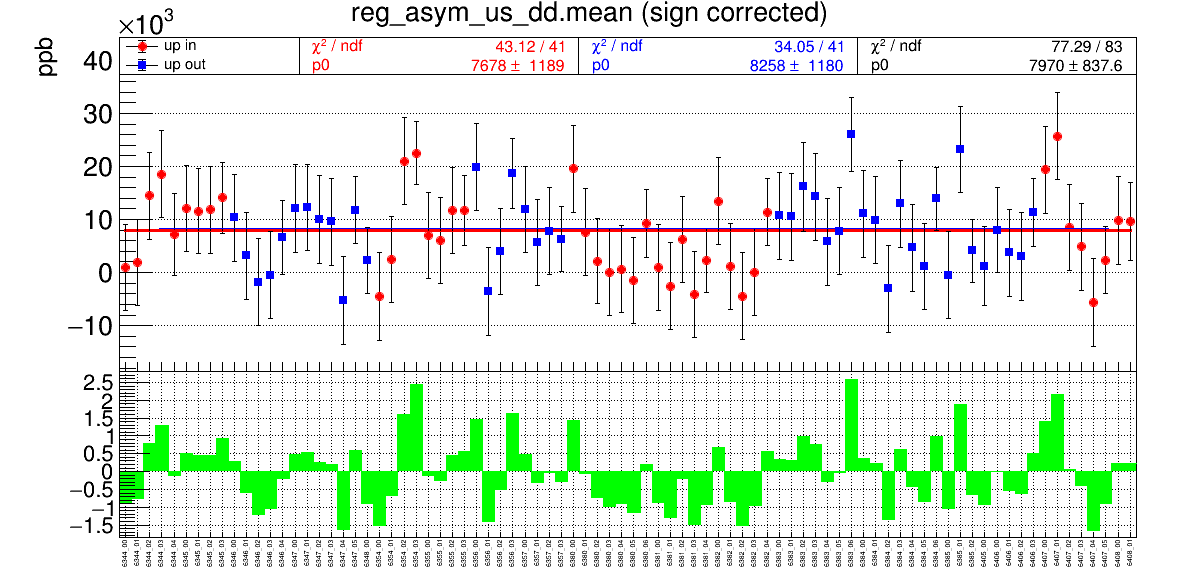
\includegraphics[width=0.9\linewidth]{at/mini_Ca48_reg_asym_us_dd.mean.png}
    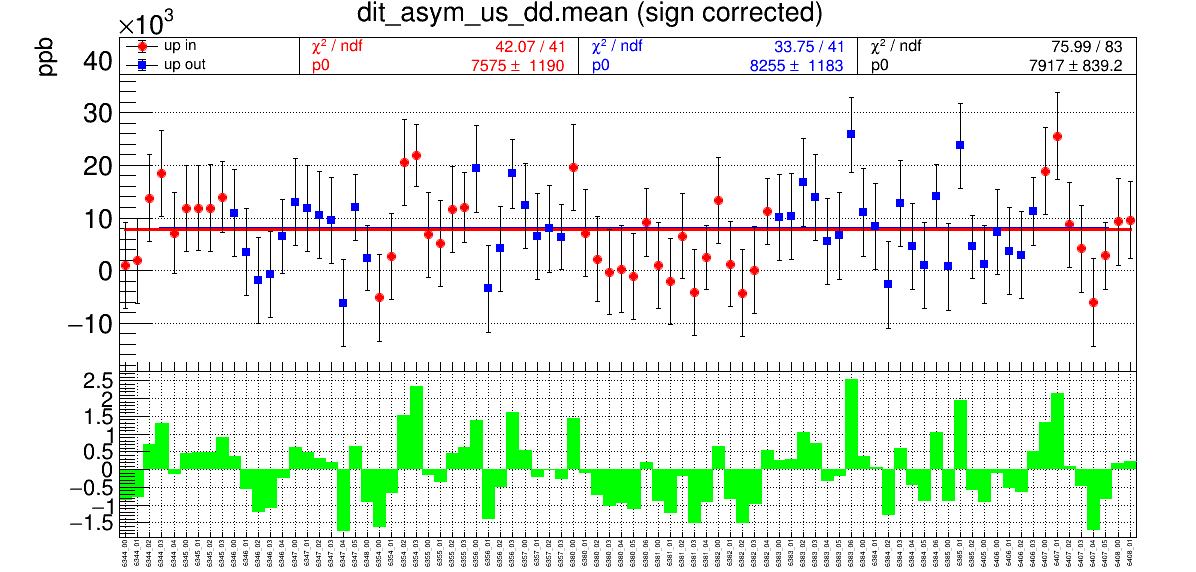
\includegraphics[width=0.9\linewidth]{at/mini_Ca48_dit_asym_us_dd.mean.png}
    \caption{Sign corrected minirun-wise scatter plot of the raw, regression corrected and 
    dithering corrected transverse asymmetry of \Ca in CREX. Different colors represent
    different IHWP states (in/out). In each plot, the top pad shows the 
    mean and error of the title variable for each minirun, the three fit lines indicate
    the zero order polynomial fit to IHWP=in, IHWP=out and all datapoints respectively;
    the bottom pad is the pull histogram, which is the ratio of the deviation 
    from the mean value of all datapoints over each datapoint's error.
    % Regress with the following 5 BPMs: bpm1X, bpm4aY, bpm4eX, bpm4eY, bpm12X.
    % PREX-regression bpms: bpm4aX/Y, bpm4eX/Y, bpmE
    }
    \label{fig:AT_crex_Ca48_miniruns}
\end{figure}


The minirun mean and mulplot mean for each target are summarized in the following
tables.
\begin{table}[!h]
    \scriptsize
    \begin{tabular}{c | r@{ $\pm$ }l r@{ $\pm$ }l r@{ $\pm$ }l | r@{ $\pm$ }l r@{ $\pm$ }l r@{ $\pm$ }l}
	\hline
	\multirow{2}{*}{Target}	& \multicolumn{6}{c|}{Minirun Average (ppb)} & \multicolumn{6}{c}{Mulplot (ppb)}	\\
	\cline{2-13}
	    & \multicolumn{2}{c}{raw}   & \multicolumn{2}{c}{reg}	& \multicolumn{2}{c|}{dit}   & \multicolumn{2}{c}{raw}	& \multicolumn{2}{c}{reg}   & \multicolumn{2}{c}{dit}	\\
	\hline
	\multicolumn{13}{c}{IHWP IN}   \\
	\hline
	\C	& 4205.3	& 1113.7    & 5173.9	& 501.5	    & 5169.4	& 502.1	    & 4129.8  & 1117.7    & 5105.0  & 504.9     & 5103.5  & 505.6   \\ 
	\ca	& 3055.9	& 1762.7    & 5507.5	& 419.3     & 5517.4	& 420.7	    & 2979.8  & 1763.3    & 5501.8  & 420.0     & 5511.7  & 421.4   \\   
	\Pb	& -266.2	& 974.2     & 54.9  	& 183.5     & 27.7  	& 185.7	    & -386.2  & 958.3     & 101.5   & 180.3     & 70.2    & 182.5   \\   
	\hline
	\multicolumn{13}{c}{IHWP OUT}   \\
	\hline
	\C	& 6111.0	& 992.1	    & 5685.5	& 437.4	    & 5740.6	& 437.9	    & 6055.9  & 995.8     & 5619.1  & 440.1     & 5669.4  & 440.6   \\ 
	\ca	& 5707.4	& 1687.6    & -679.8	& 443.0     & 5093.7	& 399.6	    & 5775.6  & 1687.8    & 5033.6  & 396.7     & 5033.6  & 399.2   \\   
	\Pb	& -132.7	& 927.4     & -52.3 	& 176.1     & -26.1 	& 178.7	    & -86.5   & 922.7     & -73.2   & 174.9     & -86.2   & 209.0   \\   
	\hline
	\multicolumn{13}{c}{COMBINED}   \\
	\hline
	\C	& 5267.8	& 740.8	    & 5464.5	& 329.6	    & 5493.9	& 330.0	    & 5209.7  & 743.5     & 5393.2  & 331.8     & 5427.0  & 332.2   \\ 
	\ca	& 4439.2	& 1219.0    & 5276.3	& 288.3     & 5294.7	& 289.7	    & 4444.9  & 1219.7    & 5275.3  & 288.5     & 5293.9  & 290.0   \\   
	\Pb	& -196.2	& 671.7     & -0.9  	& 127.0     & -0.3  	& 128.8	    & -231.5  & 664.7     & 11.3    & 125.5     & 70.2    & 182.5   \\   
	\hline
    \end{tabular}
    \caption{PREX-II raw and corrected transverse asymmetry}
\end{table}

\begin{table}[!h]
    \scriptsize
    \begin{tabular}{c | r@{ $\pm$ }l r@{ $\pm$ }l r@{ $\pm$ }l | r@{ $\pm$ }l r@{ $\pm$ }l r@{ $\pm$ }l}
	\hline
	\multirow{2}{*}{Target}	& \multicolumn{6}{c|}{Minirun Average (ppb)} & \multicolumn{6}{c}{Mulplot (ppb)}	\\
	\cline{2-13}
	    & \multicolumn{2}{c}{raw}   & \multicolumn{2}{c}{reg}	& \multicolumn{2}{c|}{dit}   & \multicolumn{2}{c}{raw}	& \multicolumn{2}{c}{reg}   & \multicolumn{2}{c}{dit}	\\
	\hline
	\multicolumn{13}{c}{IHWP IN}   \\
	\hline
	\C	& 6815.5    & 1397.2	& 7767.7    & 1182.2	& 7660.5    & 1183.4	& 6885.1    & 1397.9	& 7725.7    & 1182.1	& 7618.8 & 1183.3	\\ 
	\ca     & 8661.9    & 1643.5	& 8777.5    & 1265.2	& 8764.4    & 1267.5	& 8581.7    & 1645.3	& 8743.9    & 1265.3	& 8733.3 & 1267.6	\\ 
	\Ca     & 8306.5    & 1523.3   	& 7677.5    & 1188.9	& 7575.2    & 1190.3	& 8275.7    & 1524.9	& 7658.9    & 1189.0	& 7553.5 & 1190.3	\\ 
	\Pb	& 2742.6    & 2469.1   	& 3052.4    & 2285.9	& 3079.7    & 2288.1	& 2771.1    & 2469.6	& 3101.8    & 2286.2	& 3129.9 & 2288.3	\\ 
	\hline
	\multicolumn{13}{c}{IHWP OUT}   \\
	\hline
	\C	& 8607.9	& 1558.2    & 8789.1	& 1313.5    & 8791.5	& 1314.6    & 8512.9    & 1558.8	& 8778.2    & 1313.6	& 8780.0    & 1314.7	\\      
	\ca      & 8023.6	& 1751.5    & 7967.4	& 1353.3    & 7994.2	& 1355.0    & 8168.4    & 1755.1	& 7960.2    & 1353.4	& 7987.0    & 1355.2	\\      
	\Ca      & 7267.1	& 1516.3    & 8257.8	& 1180.2    & 8254.7	& 1183.3    & 7184.5    & 1517.6	& 8267.8    & 1180.3	& 8270.3    & 1183.5	\\      
	\Pb	& 2089.1	& 2456.4    & 2420.2	& 2263.4    & 2456.9	& 2266.2    & 2075.1    & 2456.8	& 2401.2    & 2263.8	& 2440.7    & 2266.6	\\      
	\hline
	\multicolumn{13}{c}{COMBINED}   \\
	\hline
	\C	& 7614.4	& 1040.3    & 8224.8	& 878.7     & 8166.8	& 879.5	    & 7600.8    & 1040.8	& 8235.1    & 878.8 	& 8177.3    & 879.6	\\      
	\Ca      & 8363.1	& 1198.5    & 8399.7	& 924.2     & 8405.0	& 925.6	    & 8377.3    & 1200.4	& 8383.5    & 924.3 	& 8390.4    & 925.7 	\\        
	\Ca  	& 7784.4	& 1074.7    & 7969.8	& 837.6     & 7916.9	& 839.2	    & 7725.4    & 1075.7	& 7974.4    & 837.7 	& 7923.5    & 839.3 	\\        
	\Pb      & 2414.2	& 1741.4    & 2733.1	& 1608.4    & 2765.3	& 1610.1    & 2422.6    & 1741.7	& 2751.0    & 1608.6	& 2784.8    & 1610.4	\\        
	\hline
    \end{tabular}
    \caption{CREX raw and corrected transverse asymmetry}
\end{table}

\begin{comment}
    & 343.4 & 154.8 & 155.1
    & 379.9 & 91.0  & 91.4
    & 493.9 & 93.0  & 94.1
    & 345.4 & 152.9 & 153.0
    & 387.2 & 91.3  & 91.9
    & 495.3 & 93.5  & 95.3
    & 344.5 & 153.7 & 153.9
    & 383.6 & 91.2  & 91.7
    & 494.5 & 93.2  & 94.6


\begin{table}
    \scriptsize
    \begin{tabular}{c | c c c | c c c}
	\hline
	\multirow{2}{*}{Target}	& \multicolumn{3}{c|}{Minirun Average (ppm)} & \multicolumn{3}{c}{Mulplot (ppm)}	\\
	\cline{2-7}
	    & raw	& reg	& dit	& raw	& reg	& dit	\\
	\hline
	\multicolumn{7}{c}{IHWP IN}   \\
	\hline
	C	& 659.82  & 558.10  & 558.71  & 659.84  & 557.97  & 558.56	\\
	Ca40    & 933.96  & 717.96  & 719.28  & 933.69  & 718.04  & 719.32	\\
	Ca48    & 994.35  & 775.30  & 776.19  & 994.78  & 775.61  & 776.50	\\
	Pb	& 1262.78 & 1168.89 & 1170.02 & 1261.95 & 1168.23 & 1169.35	\\
	\hline
	\multicolumn{7}{c}{IHWP OUT}   \\
	\hline
	C	& 8607.92 & 1558.19	& 8789.05 & 1313.51	& 8791.48 & 1314.60	 \\
	Ca40    & 8023.61 & 1751.48	& 7967.37 & 1353.29	& 7994.17 & 1355.00	 \\
	Ca48    & 7267.11 & 1516.31	& 8257.84 & 1180.23	& 8254.72 & 1183.33	 \\
	Pb	& 2089.10 & 2456.43	& 2420.15 & 2263.44	& 2456.87 & 2266.23	 \\
	\hline
	\multicolumn{7}{c}{COMBINED}   \\
	\hline
	C	& 661.92  & 558.72  & 559.27  & 661.73  & 558.75  & 559.29	\\
	Ca40    & 932.99  & 718.38  & 719.52  & 932.93  & 718.36  & 719.47	\\
	Ca48    & 996.46  & 775.93  & 777.46  & 996.67  & 776.15  & 777.63	\\
	Pb	& 1260.29 & 1163.94 & 1165.22 & 1259.54 & 1163.30 & 1164.57	\\
	\hline
    \end{tabular}
    \caption{Mini-wise average and mulplot average values for each target}
\end{table}
\end{comment}
As shown in the above tables, the final result from the two false asymmetry 
correction methods -- regression and dithering, agree with each other.
We chose the dithering corrected values to extract the transverse asymmetry.	% FIXME why?
The slug-wise plots of the transverse asymmetry are shown in Fig.~\ref{fig:AT_slug} 
\begin{figure}[!h]
    \centering
    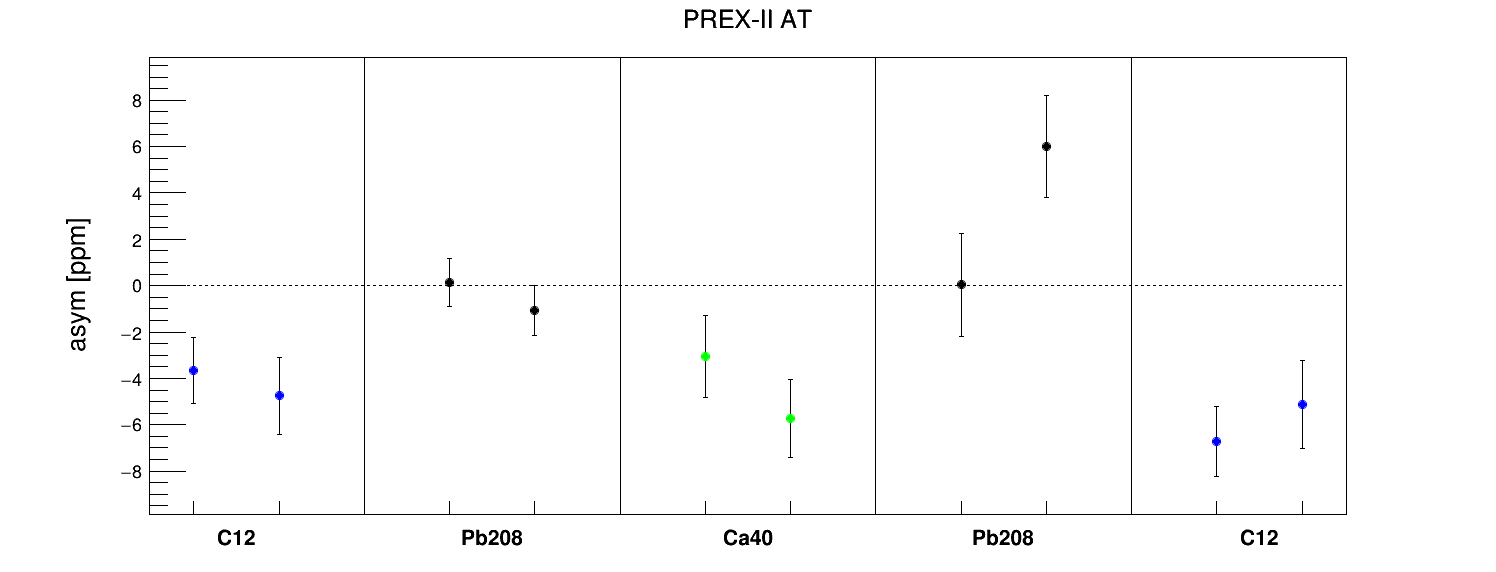
\includegraphics[width=\linewidth]{at/prex_at_slug}
    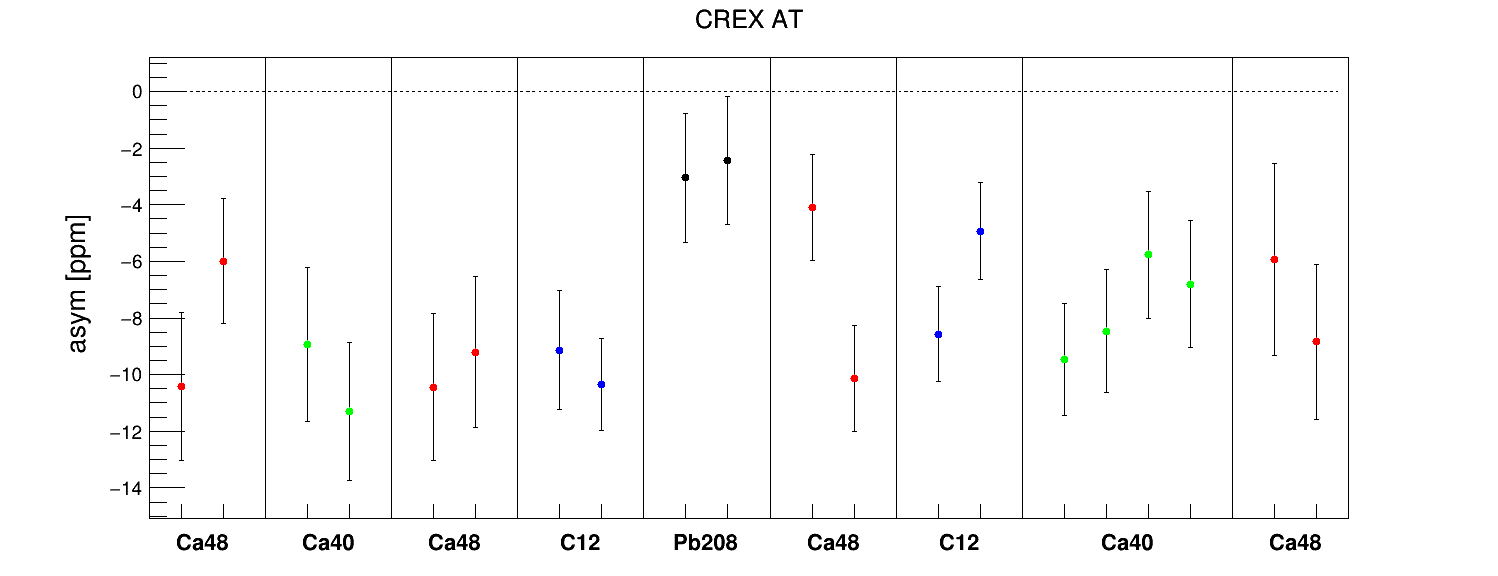
\includegraphics[width=\linewidth]{at/crex_at_slug}
    \caption{Sign corrected transverse asymmetry in chronological order. 
    Each datapoint means one slug.}
    \label{fig:AT_slug}
\end{figure}

%%%%%%%%%%%%%%%%%%%%%%%%%%%%%%%%%%%%%%%%%%%%%%%%
\subsection{Systematic Uncertainties}
Various corrections to the raw asymmetry will introduce corresponding uncertainties. 
Such as the beam false asymmetry correction, purity and detector/monitor non-linearity correction. 
These uncertainties affect the precision of the measurement, we should know 
them precisely.


%%%%%%%%%%%%%%%%%%%%%%%%
\subsubsection{Beam Correction}
% https://prex.jlab.org/DocDB/0005/000504/002/Dithering%20and%20Regression.pdf
To count the uncertainty caused by the beam correction, the difference between 
corrections with the regression and dithering methods is used. More specifically, 
we find that for most runs, the difference between the corrections
from the most significant BPMs with these two methods is less than 5\%. Therefore,
a conservative estimation of 5\% of the correction with dithering is used as the 
systematic uncertainty of the beam false asymmetry correction. 
The correction from each BPM (or their combinations) will be the product of 
the target-wise dithering slope and the average difference in each BPM (or their combinations), 
root-sum-square of 5\% of these corrections give out the uncertainty. 
The result is shown in Table~\ref{tab:beam_correction_uncertainty}.

\begin{table}[!h]
    \centering
    \begin{tabular}{c c | c c | c c | c c | c}
	\hline
	Exp & Target	
	& \multicolumn{2}{c|}{\thead{$\CA_{\text{raw}} \pm d\CA_{\text{raw}}$ \\ (ppb)}}    
	& \multicolumn{2}{c|}{\thead{$\CA_{\text{dit}}  \pm d\CA_{\text{dit}}$ \\  (ppb)}}	
	& \multicolumn{2}{c|}{\thead{$\Delta\CA \pm d(\Delta\CA)$ \\ (ppb)}}	
	& $d\Delta\CA/d\CA_{\text{dit}}$\\
	\hline
	\multirow{3}{*}{PREX-II}
	    & \C    & -5268	& 741	& -5494	& 330	& 226.1	& 29.4	& 9\%	\\ 
	    & \ca   & -4439	& 1219	& -5295	& 290	& 195.9 & 42.4	& 15\%	\\ 
	    & \Pb   & 196.2	& 672	& 0.257	& 129	& 855.5 & 71.0	& 55\%	\\ 
	\hline
	\multirow{4}{*}{CREX}
	    & \C    & -7614	& 1040	& -8167	& 880	& 552.4 & 37.8	& 4\%	\\ 
	    & \ca   & -8363	& 1198	& -8405	& 926	& 351.1 & 48.9	& 5.3\%	\\ 
	    & \Ca   & -7784	& 1075	& -7917	& 839	& 41.9  & 86.7	& 10\%	\\ 
	    & \Pb   & -2414	& 1741	& -2765	& 1610	& 132.5 & 27.8	& 2\%	\\ 
	\hline
    \end{tabular}
    \caption{Beam correction to transverse asymmetry.}
    \label{tab:beam_correction_uncertainty}
\end{table}

%%%%%%%%%%%%%%%%%%%%%%%%
\subsubsection{Purity Correction}
For the target purity correction, we need to consider only the \Pb and \Ca target.
As we will discuss in the following chapter, the contamination in the \Pb target
come from the diamond foils sandwiching the \Pb foil to cool the target, while
the impurity in \Ca target is mainly the \ca isotope. The \ca target has an abundance
larger than 99.6\%, so it is regarded as a pure target.

\begin{equation}
    \begin{gathered}
	\CA_{\text{mea}} = \frac{R_t\CA_t + \sum_i R_i \CA_i}{R_t + \sum_i R_i} = \frac{\CA_t + \sum_i f_i \CA_i}{1 + \sum_i f_i}  \\
	\CA_t = (1 + \sum_i f_i)\CA_{\text{mea}} - \sum_i f_i\CA_i
    \end{gathered}
    \label{eq:AT-asymmetry_correction}
\end{equation}
where $R$ and $\CA$ are the scattering rate and asymmetry of each nucleus, the
subscript $t$ and $i$ refer to the target and various impurity elements in the target, 
$f_i = \frac{R_i}{R_t}$ is the rate fraction. 
We use simulations to calculate the scattering rate for each different
target, asymmetry value comes from the measurement. The diamond (C) rate fraction
in the \Pb target is:
\begin{equation}
    f_C = \frac{R_C}{R_{Pb}} = 
    \begin{cases}
	0.0671 \pm 0.0057   & E = 0.95\ GeV	\\
	0.6089 \pm 0.0609   & E = 2.2\ GeV	\\
    \end{cases}
\end{equation}

The \Ca case is a little complicated, because the \Ca target is a stack of 3 different
pieces with different purities. The upstream 2 pieces are the remnant of the damaged
old target with a \Ca abundance of 95.99\%, the downstream piece is a new foil
with a \Ca abundance of 90.04\%. Based on the fact that the contamination mainly
come from various isotopes of \Ca: \ca ($\sim10\%$), ${}^{42}$Ca ($\sim0.1\%$) and ${}^{44}$Ca ($\sim0.2\%$), 
whose scattering rates and asymmetries are similar to that of \Ca, so we simplily 
count the non-\Ca fraction in the \Ca target, which leads to:
\begin{equation}
    f(\frac{non-{}^{48}Ca}{{}^{48}Ca}) = 9.07 \pm 0.18 \%
\end{equation}

Using equation \ref{eq:AT-asymmetry_correction}, the asymmetry after the purity correction
is shown in Table~\ref{tab:purity_corrected_asymmetry} .
\begin{table}
% https://docs.google.com/spreadsheets/d/1ZI68PgAn_zySKozZ__kHBvxlBmaTMKw9jPSl-EIa91k/edit?pli=1#gid=1243115322
% why cell J4 doesn't follow error propagation
% K3-K9: the formula looks weird
    \centering
    \begin{tabular}{c c | c c }
	\hline
	Exp & Target	
	& \multicolumn{2}{c}{$\CA_{\text{cor}}  \pm d\CA_{\text{stat}}$ (ppb)}	    \\
	\hline
	\multirow{3}{*}{PREX-II}
	    & \C    & -5494	& 330	 \\ 
	    & \Ca   & -5295	& 290	 \\ 
	    & \Pb   & 369	& 137	 \\ 
	\hline
	\multirow{4}{*}{CREX}
	    & \C    & -8167	& 880	 \\ 
	    & \ca   & -8405	& 926	 \\ 
	    & \Ca   & -7873	& 919	 \\ 
	    & \Pb   & 523	& 2646	 \\ 
	\hline
    \end{tabular}
    \caption{Purity corrected transverse asymmetry. The statistical uncertainties
    are calculated following the uncertainty propagation equation.}
    \label{tab:purity_corrected_asymmetry}
\end{table}

%%%%%%%%%%%%%%%%%%%%%%%%
\subsubsection{Detector Non-linearity}
For the uncertainty caused by the non-linearity in detector's response to the incoming electron flux,
it is bounded to be $<0.5\%$ in bench tests.
\begin{table}[!h]
    \centering
    \begin{tabular}{c c | c c c}
	\hline
	Exp & Target	& $\CA_{\text{raw}}$ (ppb) & $d\CA_{\text{sys}}$ (ppb)    & $\frac{d\CA_{\text{sys}}}{\CA_{\text{raw}}}$   \\
	\hline
	\multirow{3}{*}{PREX-II}
	    & \C    & -5268	& 26	& 0.50\%    \\ 
	    & \ca   & -4439	& 22	& 0.50\%    \\ 
	    & \Pb   & 196.2	& 1	& 0.50\%    \\ 
	\hline
	\multirow{4}{*}{CREX}
	    & \C    & -7614	& 38	& 0.50\%    \\ 
	    & \ca   & -8363	& 42	& 0.50\%    \\ 
	    & \Ca   & -7784	& 39	& 0.50\%    \\ 
	    & \Pb   & -2414	& 12	& 0.50\%    \\ 
	\hline
    \end{tabular}
    \caption{Systematic uncertainty due to the detector non-linearity.}
\end{table}

For uncertainty come from the BCM non-linearity, a conservative estimation of 1\% is used,
as shown in Table~\ref{tab:AT_bcm_non-linearity}, the charge asymmetry is the 
minirun-wise average value.
\begin{table}[!h]
    \centering
    \begin{tabular}{c c | c c c}
	\hline
	Exp & Target	& $\CA_{q}$ (ppb) & $d\CA_{q}$ (ppb)    & $\frac{d\CA_{q}}{\CA_{q}}$   \\
	\hline
	\multirow{3}{*}{PREX-II}
	    & \C    & -52.863   & 0.5   & 1.00\%    \\ 
	    & \ca   & -104.763  & 1.0   & 1.00\%    \\ 
	    & \Pb   & 140.602   & 1.4   & 1.00\%    \\ 
	\hline
	\multirow{4}{*}{CREX}
	    & \C    & 50.09	& 0.5   & 1.00\%    \\ 
	    & \ca   & 47.81	& 0.5   & 1.00\%    \\ 
	    & \Ca   & 27.35	& 0.3   & 1.00\%    \\ 
	    & \Pb   & -1.61	& 0.0   & 1.00\%    \\ 
	\hline
    \end{tabular}
    \caption{Systematic uncertainty due to the BCM non-linearity}
    \label{tab:AT_bcm_non-linearity}
\end{table}

%%%%%%%%%%%%%%%%%%%%%%%%%%%%%%%%%%%%%%%%%%%%%%%%
\subsection{Dynamics}

%%%%%%%%%%%%%%%%%%%%%%%%
\subsubsection{$\phi$ Angle}
% http://ace.phys.virginia.edu/HAPPEX/4179
% http://ace.phys.virginia.edu/HAPPEX/4179
It is said above that we chose the angle $\phi$ to be $90^\circ$, but no way to 
achieve exactly that value. The actually value will be a little away from
the designed value, as we measured from the data. By drawsing the $\sin\phi$ distribution
from data, the average from the distribution is taken as the measured value. 
The result is shown in the following table.
\begin{table}[!htbp]
    \centering
    \begin{tabular}{c c | c c c}
	\hline
	Exp & Target	& LHRS $\sin\phi$   & RHRS $\sin\phi$	& average   \\
	\hline
	\multirow{3}{*}{PREX-II}
	    & \C    & 0.96660   & 0.96700	& 0.9668    \\ 
	    & \ca   & 0.96430   & 0.96440	& 0.9644    \\ 
	    & \Pb   & 0.96625   & 0.96665	& 0.9665    \\ 
	\hline
	\multirow{4}{*}{CREX}
	    & \C    & 0.96950   & 0.96790	& 0.9687    \\ 
	    & \ca   & 0.97090   & 0.96920	& 0.9701    \\ 
	    & \Ca   & 0.97110   & 0.96880	& 0.9700    \\ 
	    & \Pb   & 0.96980   & 0.96830	& 0.9691    \\ 
	\hline
    \end{tabular}
    \caption{Average $\sin\phi$ values for different AT targets.}
\end{table}

%%%%%%%%%%%%%%%%%%%%%%%%
\subsubsection{$Q^2$}
Similar to the extraction of the $\phi$ angle, we draw the $Q^2$ distribution for
each target, and then took the mean value. The results are shown in the
following table.
% http://ace.phys.virginia.edu/HAPPEX/4453
% http://ace.phys.virginia.edu/HAPPEX/4468
\begin{table}[!htbp]
    \centering
    \begin{tabular}{c c | r@{ $\pm$ }l | r@{ $\pm$ }l | r@{ $\pm$ }l r@{ $\pm$ }l}
	\hline
	Exp & Target	
	& \multicolumn{2}{c|}{\thead{LHRS $Q^2$ \\ ($\mathrm{GeV}^2$)}} 
	& \multicolumn{2}{c|}{\thead{RHRS $Q^2$ \\ ($\mathrm{GeV}^2$)}} 
	& \multicolumn{2}{c}{\thead{Average $Q^2$ \\ ($\mathrm{GeV}^2$)}} & \multicolumn{2}{c}{\thead{Average $Q$ \\ ($\mathrm{GeV}$)}} \\
	\hline
	\multirow{4}{*}{PREX-II}
	& \C	& 0.0068    & 4E-6  & 0.0066    & 5E-6	& 0.00671   & 3.21E-6	& 0.082	& 1.96E-5	\\
	& \ca  	& 0.0068    & 5E-6  & 0.0067    & 6E-6  & 0.00673   & 4.17E-6  & 0.082	& 2.54E-5	\\
	& \Pb 8	& 0.0065    & 5E-6  & 0.0063    & 6E-6  & 0.00640   & 4.06E-6  & 0.080	& 2.54E-5	\\
	& \Pb 9	& 0.0065    & 4E-6  & 0.0063    & 5E-6  & 0.00640   & 3.50E-6  & 0.080	& 2.18E-5	\\
	\hline
	\multirow{4}{*}{CREX}
	& \C	& 0.0328    & 2E-5  & 0.0334    & 2E-5	& 0.0331    & 1.31E-5  & 0.182	& 3.61E-5	\\
	& \ca  	& 0.0306    & 2E-5  & 0.0309    & 2E-5	& 0.0308    & 1.22E-5  & 0.175	& 3.48E-5	\\
	& \Ca  	& 0.0304    & 1E-5  & 0.0307    & 2E-5	& 0.0306    & 1.07E-5  & 0.175	& 3.05E-5	\\
	& \Pb	& 0.0319    & 3E-5  & 0.0322    & 3E-5	& 0.0320    & 1.99E-5  & 0.179	& 5.56E-5	\\
	\hline
    \end{tabular}
    \caption{Average $Q^2$ values for different AT targets.}
\end{table}

%%%%%%%%%%%%%%%%%%%%%%%%%%%%%%%%%%%%%%%%%%%%%%%%
\subsection{Final Result}
With Eq.~\ref{eq:measured_AT}, the transverse asymmetry is calculated to be:
\begin{equation}
    \CA_n = \frac{\CA_{\text{cor}}}{\CP_n \cdot \sin\phi}
\end{equation}

The statistical uncertainty is:
\begin{equation}
    d\CA_n(\text{stat}) = \frac{d\CA_{\text{cor}}(\text{stat})}{\CP_n \cdot \sin\phi}
\end{equation}
and the systematic uncertainty is:
\begin{equation}
    \left( \frac{d\CA_n(\text{sys})}{\CA_n} \right)^2 = 
	\left( \frac{d\CA_{\text{cor}}(\text{sys})}{d\CA_{\text{cor}}} \right)^2
	+ \left( \frac{d\CP_n}{\CP_n}\right)^2 
\end{equation}
where
\begin{equation}
    d\CA^2_{\text{cor}}(\text{sys}) = d\CA^2(\text{det\ nonlin}) + d\CA^2(\text{BCM\ nonlin}) + d\CA^2(\text{beam\ correction})
\end{equation}
For the \Pb and \Ca target, we need to include uncertainties from contaminations.
Various systematic uncertainties are summarized in Table~\ref{tab:AT_uncertainties}.
\begin{table}[!h]
    \centering
    \begin{tabular}{c c c c | c c c c}
	\hline
	Exp & \multicolumn{3}{c|}{PREX-II}  & \multicolumn{4}{c}{CREX}	\\
	Target	& \C	& \ca	& \Pb	& \C	& \ca	& \Ca	& \Pb	\\
	\hline
	Beam correction & 0.03  & 0.05  & 0.08  & 0.04  & 0.06  & 0.10  & 0.03	\\
	Polarization    & 0.06  & 0.05  & $<0.01$ & 0.08  & 0.08  & 0.08  & $<0.01$	\\
	Non-linearity   & 0.03  & 0.03  & $<0.01$ & 0.05  & 0.05  & 0.05  & 0.01	\\
	Tgt. impurity   & $<0.01$ & $<0.01$ & 0.04  & $<0.01$ & $<0.01$ & 0.10  & 0.80	\\
	Inelastic	& $<0.01$ & $<0.01$ & $<0.01$ & 0.08  & 0.15  & 0.08  & $<0.01$	\\
	\hline	
	Tot. Syst	& 0.07  & 0.08  & 0.09  & 0.13  & 0.18  & 0.19  & 0.75	\\
	Statistical	& 0.38  & 0.34  & 0.16  & 1.05  & 1.10  & 1.09  & 3.15	\\
	Total		& 0.39  & 0.34  & 0.18  & 1.05  & 1.11  & 1.11  & 3.23	\\
	\hline
    \end{tabular}
    \caption{AT uncertainty contributions in units of ppm}
    \label{tab:AT_uncertainties}
\end{table}

The final result is shown in Table~\ref{tab:AT_final_values}:
\begin{table}[!h]
    \centering
    \begin{tabular}{c c | c c c c}
	\hline
	Exp & Target	& \thead{$\CA_n$ \\ (ppm)}   & \thead{$d\CA_{stat}$ \\ (ppm)}	
	& \thead{$d\CA_{sys}$ \\ (ppm)}	& \thead{$d\CA_{stat+sys}$ \\ (ppm)}	\\
	\hline
	\multirow{3}{*}{PREX-II}
	    & \C    & -6.34	& 0.38	& 0.07	& 0.39	\\ 
	    & \ca   & -6.12	& 0.34	& 0.08	& 0.34	\\ 
	    & \Pb   & 0.43	& 0.16	& 0.09	& 0.18	\\ 
	\hline
	\multirow{4}{*}{CREX}
	    & \C    & -9.71	& 1.05	& 0.10	& 1.05	\\ 
	    & \ca   & -9.98	& 1.10	& 0.11	& 1.11	\\ 
	    & \Ca   & -9.35	& 1.09	& 0.17	& 1.11	\\ 
	    & \Pb   & 0.62	& 3.15	& 0.75	& 3.23	\\ 
	\hline
    \end{tabular}
    \caption{Final result of the transverse asymmetry.}
    \label{tab:AT_final_values}
\end{table}

Comparing to the theoretical calculations \cite{PhysRevC.103.064316}, we confirm 
the anomaly appeared in PREX-I AT measurement, that is the \Pb transverse asymmetries
are consistently 0 at various $Q$ values, as shown in Fig.~\ref{fig:pcrex_AT}. 
As for other light nuclei, they are not far away from their theoretical predictions.
\begin{figure}[!h]
    \centering
    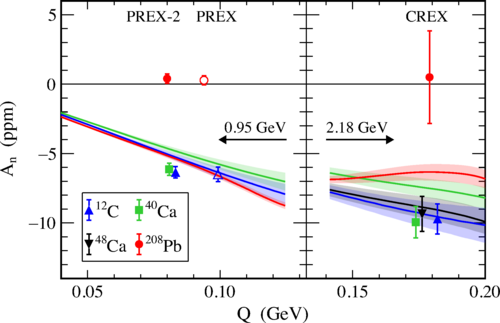
\includegraphics[scale=.5]{at/pcrex_AT}
    \caption{Transverse asymmetries measured in PREX-II/CREX. The PREX-I result
    is also included. Overlapping points are offset slightly in Q to distinguish
    them.}
    \label{fig:pcrex_AT}
\end{figure}

\begin{comment}
    \begin{itemize}
	\item resource: AT plot: https://github.com/cipriangal/prexATplot
	\item regression: which bpm set were used?
	\item dithering: ???
	\item 
    \end{itemize}
\end{comment}
